\documentclass[a4paper,12pt]{article}

% Character set
\usepackage{cmap}
\usepackage[utf8]{inputenc}
\usepackage[T1]{fontenc} % ensure that all the characters in characterSets.tex prints
\usepackage{upquote} % \textcent
\usepackage{pifont} % add \ding, http://ctan.org/pkg/pifont

% A background text to prevent wide distribution
\usepackage{draftwatermark}
\SetWatermarkText{DRAFT}
\SetWatermarkScale{6}
\SetWatermarkLightness{.95}

% Page setup
\usepackage[top=25mm,bottom=20mm,inner=20mm,outer=40mm,marginparsep=3mm,marginparwidth=35mm]{geometry}
\renewcommand{\floatpagefraction}{.8}%

% paragraph indentation is stupid
\setlength\parindent{0pt}
\setlength{\parskip}{1em}

% Globally defined colors
\usepackage[table,x11names]{xcolor}
\definecolor{alternateKeywordsColor}{rgb}{0.13,1,0.13}
\definecolor{keywordsColor}{rgb}{0.13,0.13,1}
%\definecolor{commentsColor}{rgb}{0,0.5,0}
\definecolor{commentsColor}{rgb}{0,0.5,0}
%\definecolor{stringsColor}{rgb}{0.9,0,0}
\definecolor{stringsColor}{rgb}{0,0,0.5}
\definecolor{light-gray}{gray}{0.95}
\definecolor{codeLineHighlight}{named}{SlateGray1}
%\definecolor{codeLineHighlight}{rgb}{0.975,0.975,0.975}
\definecolor{syntaxColor}{rgb}{0,.45,0}

\definecolor{headerRowColor}{rgb}{0.85,0.85,0.85}
\definecolor{oddRowColor}{rgb}{0.95,0.95,0.95}
\definecolor{evenRowColor}{rgb}{1,1,1}

% add check- and crossmarks, http://ctan.org/pkg/pifont
\newcommand{\cmark}{{\color{green}\ding{51}}}%
\newcommand{\xmark}{{\color{red}\ding{55}}}%

% Extra math stuff
\usepackage{amsmath,amssymb}

% Typeset chess
\usepackage{skak}

% Figures
\usepackage{graphicx}
\graphicspath{{figures/}}

% clickable url
\usepackage{url}

% figures
\usepackage{subfigure}

% Clickable table of content
\usepackage[pdfpagelabels]{hyperref}
%\usepackage{multirow}
\usepackage{makecell}

% Include label name in ref
\usepackage[noabbrev,capitalize]{cleveref}
\newcommand{\creflastconjunction}{, and\nobreakspace~}
\Crefformat{tcb@cnt@codeNOutput}{Listing~#2#1#3}
\crefformat{tcb@cnt@codeNOutput}{Listing~#2#1#3}
\crefrangeformat{tcb@cnt@codeNOutput}{Listing~#3#1#4\nobreakdash--#5#2#6}
\Crefrangeformat{tcb@cnt@codeNOutput}{Listing~#3#1#4\nobreakdash--#5#2#6}
\crefmultiformat{tcb@cnt@codeNOutput}{Listing~#2#1#3}{ and~#2#1#3}{, #2#1#3}{\creflastconjunction#2#1#3}
\Crefmultiformat{tcb@cnt@codeNOutput}{Listing~#2#1#3}{ and~#2#1#3}{, #2#1#3}{\creflastconjunction#2#1#3}
\crefrangeformat{table}{Table~#3#1#4\nobreakdash--#5#2#6}
\Crefrangeformat{table}{Table~#3#1#4\nobreakdash--#5#2#6}
\crefrangeformat{part}{Part~#3#1#4\nobreakdash--#5#2#6}
\Crefrangeformat{part}{Part~#3#1#4\nobreakdash--#5#2#6}

% paragraphs in tables
\usepackage{tabularx}

% formatting lists
\usepackage{enumitem}
%\setlist[description]{leftmargin=0pt,labelindent=0pt,itemindent=0pt}
%\setlist[description]{itemindent=-\leftmargin}

% latex comment environment
\usepackage{comment}

% UML
\usepackage{pgf-umlcd}
\renewcommand{\umltextcolor}{black} 
\renewcommand{\umlfillcolor}{black!5!white}
\renewcommand{\umldrawcolor}{teal}

% List of indices
\usepackage{xstring}
\usepackage{makeidx}
\usepackage{marginfix} % fixes marginpar location problem in 2 -page mode.
\newcommand{\idxs}[1]{\marginpar{$\cdot$~\parbox[t]{\linewidth}{\raggedright \expandarg\IfSubStr{#1}{@}{\StrBehind{#1}{@}}{#1}}}\index{#1}} % The parbox is too wide, since the line also includes cdot-space
\newcommand{\idxss}[1]{\index{#1}}
% Define a new command idx with an optional parameter, which if given is the key to the index
\makeatletter
\def\idx{\@ifnextchar[{\@with}{\@without}}
\def\@with[#1]#2{\emph{#2}\idxs{#1}}
\def\@without#1{\emph{#1}\idxs{#1}}
\makeatother
%\newcommand{\idx}[1]{\emph{#1}\idxs{#1}}
\newcommand{\keyword}[1]{{\lstinline[language=fsharp]|#1|}}
\newcommand{\lexeme}[1]{\mbox{``\lstinline[language=fsharp]|#1|''}}
\makeindex

% display tree like structures
\usepackage{qtree}

% We frame all listings and problems
\usepackage{tcolorbox}
\tcbuselibrary{listings}
\tcbuselibrary{raster}
\tcbset{%
  colframe=teal, %PaleGreen1!45!black,
  %coltitle=black,
  fonttitle=\bfseries, 
  leftrule=3mm,
  sharp corners=downhill,
  colback=black!5!white,
  left=1mm,
  top=1mm,
  right=1mm,
  bottom=1mm,
  middle=1mm,
  arc=2mm,
}
\newtcolorbox[auto counter]{problem}[1][]{%
  title=\textbf{Problem~\thetcbcounter},
  colframe=DeepSkyBlue1, %green!30!blue,
  #1}
\newcommand{\src}{src}
\newtcolorbox[auto counter]{codeNOutput}[2][]{%
  title=\textbf{Listing~\thetcbcounter#2},
  #1}

%% lstlisting stuff
\usepackage{listings} 
\def\lstfs#1{\mbox{\lstinline{{#1}}}}
% Get counters from references for firstnumber references in lstinputlisting
\usepackage{refcount}
\newcounter{lstFrom}
\newcounter{lstTo}
% Example: 
% \setcounterref{lstFrom}{dynamicScopeTracing:a1}
% \setcounterref{lstTo}{dynamicScopeTracing:a2}
% \lstinputlisting[firstline=\thelstFrom,lastline=\thelstTo,escapechar=|]{\src/dynamicScopeTracing.fsx}
\usepackage{lstlinebgrd}
\makeatletter
%The following sets the box compatible with tcolorbox setup
\def\lst@linebgrdcolor{\color{black!5!white}}
\def\lst@linebgrdsep{1em}
\def\lst@linebackgroundwidth{1em}
\def\lst@linebackgroundhighlight{\color{codeLineHighlight}}
\renewcommand{\lst@linebgrd}{%
  \ifx\lst@linebgrdcolor\empty
  \else
    \rlap{
       \lst@basicstyle\color{black!5!white} % tcolorbox background color
       \lst@linebgrdcolor{
          \kern-\dimexpr\lst@linebgrdsep\relax
          \lst@linebgrdcmd{\lst@linebgrdwidth}{\lst@linebgrdheight}{\lst@linebgrddepth}
       }
    }
  \fi
}
% Highlight a range of lines with green. Use \getrefnumber{label} for refs
\newcommand{\highlightRange}[2]{\ifnum\value{lstnumber}>\numexpr#1-1\ifnum\value{lstnumber}<\numexpr1+#2\lst@linebackgroundhighlight\fi\fi}
% \highlight conflicts with skak. Just rewriting, wonder what breaks in skak
\renewcommand{\highlight}[1]{\ifnum\value{lstnumber}=#1\lst@linebackgroundhighlight\fi}

% To use verbatimwrite to write listing to file, e.g., in conjunction with ebnfs
\usepackage{moreverb} 

\lstdefinelanguage{fsharp}{%
  keywords={abstract, and, as, assert, base, begin, class, default, delegate, do, done, downcast, downto, elif, else, end, exception, extern, false, finally, for, fun, function, global, if, in, inherit, inline, interface, internal, lazy, let, match, member, module, mutable, namespace, new, null, of, open, or, override, private, public, rec, return, sig, static, struct, then, to, true, try, type, upcast, use, val, void, when, while, with, yield},
  morekeywords={atomic, break, checked, component, const, constraint, constructor, continue, eager, fixed, fori, functor, include, measure, method, mixin, object, parallel, params, process, protected, pure, recursive, sealed, tailcall, trait, virtual, volatile},
  otherkeywords={ let!, return!, do!, yield!, use!},
  keywordstyle=\color{keywordsColor},
  % sensitive=true,
  basicstyle=\ttfamily\lst@ifdisplaystyle\small\fi, % make font small for listings but not for lstinline
  breaklines=true,
  breakatwhitespace=true
  showstringspaces=false,
  morecomment=[l][\color{commentsColor}]{///},
  morecomment=[l][\color{commentsColor}]{//},
  morecomment=[n][\color{commentsColor}]{(*}{*)},
  morecomment=[is][\color{white}]{(*//}{*)},
  morestring=[b]",
  literate={`}{\`}1,
  stringstyle=\color{stringsColor},
  showspaces=true,
  numbers=left,
  numbersep=6pt,
  numberstyle=\scriptsize\color{white},
  % aboveskip=0pt, 
  % belowskip=0pt,
  % resetmargins=true,
  % captionpos=b,
  backgroundcolor=\color{black!5!white},
}


\lstdefinelanguage{syntax}{%
  classoffset=0,
  keywords={abstract, and, as, assert, base, begin, class, default, delegate, do, done, downcast, downto, elif, else, end, exception, extern, false, finally, for, fun, function, global, if, in, inherit, inline, interface, internal, lazy, let, match, member, module, mutable, namespace, new, null, of, open, or, override, private, public, rec, return, sig, static, struct, then, to, true, try, type, upcast, use, val, void, when, while, with, yield, atomic, break, checked, component, const, constraint, constructor, continue, eager, fixed, fori, functor, include, measure, method, mixin, object, parallel, params, process, protected, pure, recursive, sealed, tailcall, trait, virtual, volatile, let!, return!, do!, yield!, use!},
  keywordstyle=\color{keywordsColor},
  % classoffset=1,
  % morekeywords={ident, expr, arg, format-string},
  % keywordstyle=\color{syntaxColor},
  % classoffset=0,
  otherkeywords={},
  basicstyle=\ttfamily\lst@ifdisplaystyle\small\fi, % make font small for listings but not for lstinline
  breaklines=true,
  breakatwhitespace=true
  showstringspaces=false,
  classoffset=0,
  morecomment=[l][\color{commentsColor}]{////},
  literate={`}{\`}1 {\{*}{{{\color{syntaxColor}\{}}}1 {*\}}{{{\color{syntaxColor}\}}}}1 {[*}{{{\color{syntaxColor}[}}}1  {*]}{{{\color{syntaxColor}]}}}1 {|*}{{{\color{syntaxColor}|}}}1, % {etc*}{{{\color{syntaxColor}...}}}3,
  moredelim  = **[is][\processmydelims]{<*}{*>}, % delete delimiters, typeset keywords. Don't know how to avoid the last...
  showspaces=true,
  numbers=left,
  numbersep=6pt,
  numberstyle=\scriptsize\color{white},
  backgroundcolor=\color{black!5!white},
}
%Tweek of deliminter and literate: https://tex.stackexchange.com/questions/203263/listings-package-custom-language-delimiter-match-left-side
\newcommand\processmydelimsend{}
\newcommand\processmydelims{%
  \renewcommand\processmydelimsend{\textcolor{syntaxColor}{>}\egroup}%
  \bgroup\color{syntaxColor}<\aftergroup\processmydelimsend%
}
% \makeatletter
% \newcommand\processhash{%
%   \ifnum\lst@mode=\lst@Pmode%
%     \bfseries%
%   \fi
%   \#%
% }
% \makeatother


\lstdefinelanguage{ebnf}{%
  keywords={},
  morekeywords={},
  otherkeywords={},
  keywordstyle=\color{keywordsColor},
  % sensitive=true,
  basicstyle=\fontfamily{pcr}\selectfont\lst@ifdisplaystyle\small\fi, 
  breaklines=true,
  breakatwhitespace=true
  morecomment=[s][\color{commentsColor}]{(*}{*)},
  morestring=[b]",
  morestring=[b]',
  alsoletter={\\},
  showstringspaces=false,
  % stringstyle=\color{stringsColor},
  % aboveskip=0pt, 
  % belowskip=0pt,
  % resetmargins=true,
  % captionpos=b,
  % backgroundcolor=\color{blue!10!white},
}
\lstdefinelanguage{console}{%
  keywords={},
  morekeywords={},
  otherkeywords={},
  basicstyle=\ttfamily\lst@ifdisplaystyle\small\fi, 
  breaklines=true,
  showstringspaces=false,
  % aboveskip=0pt,
  % belowskip=0pt,
  % resetmargins=true,
  % captionpos=b,
  % backgroundcolor=\color{green!10!white},
}
%\lstset{language=fsharp, frame=single}
\lstset{language=fsharp,showlines=false}
\makeatletter
\def\lst@visiblespace{ }
\makeatother

% input .fsx and .out listings from \src and display as code and result in same figure
% #1 = optional further arguments for lstinputlisting
% #2 = filename without suffix, and label
% #3 = caption
\newtcbinputlisting[use counter from=codeNOutput]{\fs}[3][]{%
  listing file={src/#2.fsx},
  listing and comment,
  listing options={language=fsharp,escapechar=§,#1},
  title=\textbf{Listing \thetcbcounter} {#2.fsx:\\#3},
  label={#2},
  comment={\lstinputlisting[language=console]{\src/#2.out}}
}

% dispaly fsharp code \src
% #1 = optional further arguments for lstinputlisting
% #2 = filename
% #3 = label
% #4 = caption
\newtcbinputlisting[use counter from=codeNOutput]{\fsharp}[4][]{%
  listing file={\src/#2},
  listing only,
  listing options={language=fsharp,escapechar=§,#1},
  title=\textbf{Listing \thetcbcounter} {#2:\\#4},
  label={#3},
}

% dispaly console file \src
% #1 = optional further arguments for lstinputlisting
% #2 = filename
% #3 = label
% #4 = caption
\newtcbinputlisting[use counter from=codeNOutput]{\console}[4][]{%
  listing file={\src/#2},
  listing only,
  listing options={language=console,escapechar=§,#1},
  title=\textbf{Listing \thetcbcounter} {#2:\\#4},
  label={#3},
}

\newtcbinputlisting[use counter from=codeNOutput]{\fsCode}[4]{%
  listing file={src/#1.fsx},
  listing only,
  listing options={language=fsharp,escapechar=§,#4},
  title=\textbf{Listing \thetcbcounter} {#1.fsx:\\#3},
  label={#2},
}

% dispaly ebnf file, no label
% #1 = optional further arguments for lstinputlisting
% #2 = filename
% #3 = caption
\newtcbinputlisting[use counter from=codeNOutput]{\ebnf}[3][]{%
  listing file={#2},
  listing only,
  colframe=black!50!white,
  listing options={language=ebnf,escapechar=§,#1},
  title=\textbf{Listing \thetcbcounter} {#3},
}

% dispaly syntax file, no label
% #1 = optional further arguments for lstinputlisting
% #2 = filename without suffix, and label
% #3 = caption
\newtcbinputlisting[use counter from=codeNOutput]{\syntax}[3][]{%
  listing file={#2},
  listing only,
  colframe=black!50!white,
  listing options={language=syntax,escapechar=§,#1},
  title=\textbf{Listing \thetcbcounter} {#3},
  label={#2}
}

\newtcbinputlisting[use counter from=codeNOutput]{\fsSignature}[4]{%
  listing file={src/#1.fsi},
  listing only,
  listing options={language=fsharp,escapechar=§,#4},
  title=\textbf{Listing \thetcbcounter} {#1.fsi:\\#3},
  label={#2},
}
\newtcbinputlisting[use counter from=codeNOutput]{\fsImplementation}[4]{%
  listing file={src/#1.fs},
  listing only,
  listing options={language=fsharp,escapechar=§,#4},
  title=\textbf{Listing \thetcbcounter} {#1.fs:\\#3},
  label={#2},
}

% dispaly output file .out from \src
% #1 = optional further arguments for lstinputlisting
% #2 = filename without suffix, and label
% #3 = caption
\newtcbinputlisting[use counter from=codeNOutput]{\fsOutput}[3][]{%
  listing file={src/#2.out},
  listing only,
  listing options={language=console,escapechar=§,#1},
  title=\textbf{Listing \thetcbcounter}: {#3},
  label={#2},
}

% dispaly output file .out from \src as an element in tabularx
% #1 = optional further arguments for lstinputlisting
% #2 = filename without suffix, and label
% #3 = caption
\newtcbinputlisting[use counter from=codeNOutput]{\fsOutputTabx}[3][]{%
  listing file={src/#2.out},
  listing only,
  width=\hsize,
  box align=top,
  listing options={language=console,escapechar=§,aboveskip=0pt,belowskip=0pt,emptylines=0,#1},
  title=\textbf{Listing \thetcbcounter}: {#3},
  label={#2},
}

\newcommand{\filename}[1]{\lstinline[language=console]{#1}}

% highlighted text snippets
\newcommand{\advice}[1]{\marginpar{Advice}{\textbf{#1}}}
\newcommand{\advanced}[1]{\marginpar{Advanced material}\textbf{#1}}

% sometimes we need to include hash sign as arguments
\begingroup\catcode`\#=12
\newcommand\hashchar{}%check that is doesn't exist
\gdef\hashchar{#}
\endgroup

% Scratch out math, used in test.tex
\usepackage{cancel}
%\newcommand{\bcancel}[1]{#1}

% Draw arrows between elements
\usepackage{tikz}
%\usepackage{sphack} % make overlays invisible where stated in text
\usetikzlibrary{arrows,shapes,calc,decorations.pathreplacing}
\newcommand{\tikzmark}[1]{\tikz[overlay,remember picture] \node (#1) {};}
\newcommand*{\DrawArrow}[3][]{%
  % #1 = draw options
  % #2 = left point
  % #3 = right point
  \begin{tikzpicture}[overlay,remember picture]
    %\draw [-latex, #1,ultra thick,red] ($(#2)+(0.1em,0.5ex)$) to ($(#3)+(0,0.5ex)$);
    \draw [-latex, #1,ultra thick,red] ($(#2) -(0,0.5ex)$) to ($(#3)+(0,2ex)$);
  \end{tikzpicture}%
}%
\newcommand*{\AddNote}[4]{%
  \begin{tikzpicture}[overlay, remember picture]
    \draw [decoration={brace,amplitude=0.5em},decorate,ultra thick,red]
    ($(#3)!([yshift=1.5ex]#1)!($(#3)-(0,1)$)$) -- ($(#3)!(#2)!($(#3)-(0,1)$)$)
    node [align=left, text width=0cm, pos=0.5, anchor=west, xshift=.2cm] {#4};
  \end{tikzpicture}
}%
\newcommand{\FrameArea}[2]{%
  % #1 = top left point
  % #2 = bottom right point
  % The overlay is drawn in the margin in order not to screw with
  % horizontal spacing.
  %\ifvmode\vspace*{-1.2em}\else\fi%
  \begin{tikzpicture}[overlay,remember picture]%
    \draw[red,rounded corners] ([shift={(-2pt,1.9ex)}] #1)  rectangle  ([shift={(2pt,-.9ex)}] #2);%
  \end{tikzpicture}\noindent % I don't know why this command shift to the right, but this seems to fix it.
}%

% One can write to a file during compilation with the following
% low-level code.
%  \newwrite\tempfile
%  \immediate\openout\tempfile=list.tex
%  \immediate\write\tempfile{Text to write to file}
%  \immediate\closeout\tempfile

\usepackage{xspace}
\newcommand{\monoVersion}{5.2.0\xspace}
\newcommand{\fsharpVersion}{4.1\xspace}


% Notes to self
\newcommand{\jon}[1]{\footnote{Jon: \textbf{#1}}}
%\renewcommand{\jon}[1]{}
\newcommand{\mael}[1]{\footnote{Mael: \textbf{#1}}}
%\renewcommand{\mael}[1]{}
\newcommand{\spec}[1]{\footnote{Spec: \textbf{#1}}}
\renewcommand{\spec}[1]{}

%%% Local Variables:
%%% TeX-master: "fsharpNotes"
%%% End:


%\usepackage{cmap}
%\usepackage[utf8x]{inputenc}
%\usepackage{latexsym}
%\usepackage[danish]{babel}
%\usepackage{graphicx}
\usepackage{graphpap}
%\usepackage{color}
%\usepackage{hyperref}
%\usepackage[all]{hypcap}
%\usepackage{enumerate}
\usepackage{tikz}
\usetikzlibrary{patterns}

\title{Programmering og Problemløsning\\Datalogisk Institut,
  Københavns Universitet\\Arbejdsseddel 8 --- gruppeopgave}

\author{Martin Elsman\thanks{Denne opgaver er baseret på en tidligere variant af opgaven konstrueret af Torben Mogensen.}}
\date{30.\ oktober -- 29.\ november.\\Afleveringsfrist: onsdag d.\ 29.\ november kl. 22:00}

\begin{document}
\maketitle

I denne periode skal I arbejde i grupper.  Formålet er at arbejde med
sumtyper og endelige træer. Opgaverne er delt i øve- og
afleveringsopgaver.

\section*{Øveopgaver}

I de næste to opgaver skal følgende sum-type benyttes til at
repræsentere ugedage:

\begin{lstlisting}[numbers=none,frame=none,mathescape]
type weekday = Monday | Tuesday | Wednesday | Thursday
             | Friday | Saturday | Sunday
\end{lstlisting}

\begin{enumerate}[label=8ø.\arabic*,start=0]
\item Lav en funktion \texttt{dayToNumber : weekday -> int}, der givet
  en ugedag returnerer et tal, hvor mandag skal give tallet 1, tirsdag
  tallet 2 osv.

\item Lav en funktion \texttt{nextDay : weekday -> weekday}, der givet
  en ugedag returnerer den næste dag, så mandag skal give tirsdag,
  tirsdag skal give onsdag, osv, og søndag skal give mandag.
\end{enumerate}

I de følgende opgaver (både øveopgaver og
afleveringsopgaver) skal vi arbejde med en træstruktur til at beskrive geometriske
figurer med farver.  For at gøre det muligt at afprøve jeres opgaver
skal I gøre brug af det udleverede bibliotek \texttt{img\_util.dll}, der
blandt andet kan omdanne såkaldte bitmap-arrays til png-filer.  Biblioteket er
beskrevet i forelæsningerne (i uge 6) og koden for biblioteket ligger
sammen med forelæsningsplancherne for uge 6.  Her bruger vi
funktionerne til at konstruere et bitmap-array samt til at gemme
arrayet som en png-fil:

\begin{lstlisting}[numbers=none,frame=none,mathescape]
// colors
type color = System.Drawing.Color
val fromRgb : int * int * int -> color
// bitmaps
type bitmap = System.Drawing.Bitmap
val mk       : int -> int -> bitmap
val setPixel : color -> int * int -> bitmap -> unit

// save a bitmap as a png file
val toPngFile : string -> bitmap -> unit
\end{lstlisting}

Funktionen \lstinline{toPngFile} tager som det første argument navnet
på den ønskede png-fil (husk extension).  Det andet argument er
bitmap-arrayet som ønskes konverteret og gemt. Et bitmap-array kan
konstrueres med funktionen \lstinline{ImgUtil.mk}, der tager som
argumenter vidden og højden af billedet i antal pixels, samt funktionen
\lstinline{ImgUtil.setPixel}, der kan bruges til at opdatere bitmap-arrayet
før det eksporteres til en png-fil. Funktionen \lstinline{ImgUtil.setPixel}
tager tre argumenter. Det første argument repræsenterer en farve og
det andet argument repræsenterer et punkt i bitmap-arrayet (dvs.\@ i
billedet). Det tredie argument repræsenterer det bitmap-array, der
skal opdateres.  En farve kan nu konstrueres med funktionen
\lstinline{ImgUtil.fromRgb} der tager en triple af tre tal mellem 0 og
255 (begge inklusive), der beskriver hhv.\@ den røde, grønne og blå del
af farven.

Koordinaterne starter med $(0,0)$ i øverste venstre hjørne og
$(w-1,h-1)$ i nederste højre hjørne, hvis bredde og højde er hhv.\ $w$
og $h$.  Antag for eksempel at programfilen \texttt{testPNG.fsx}
indeholder følgende F\# kode:

\begin{lstlisting}[numbers=none,frame=none,mathescape]
let bmp = ImgUtil.mk 256 256
do ImgUtil.setPixel (ImgUtil.fromRgb (255,255,0)) (10,10) bmp
do ImgUtil.toPngFile "test.png" bmp
\end{lstlisting}

\noindent
Det er nu muligt at generere en png-fil med navn \texttt{test.png} ved
at køre følgende kommando:

  \vspace{-4mm}
\begin{verbatim}
  fsharpi -r img_util.dll testPNG.fsx
\end{verbatim}
  \vspace{-4mm}

\noindent
Den genererede billedfil \texttt{test.png} vil indeholde
et sort billede med et pixel af gul farve i punktet (10,10).

\noindent
Bemærk, at alle programmer, der bruger \texttt{ImgUtil} skal køres
eller oversættes med \texttt{-r img\_util.dll} som en del af
kommandoen.
%
Bemærk endvidere, at \LaTeX\ kan inkludere png-filer med
kommandoen \texttt{includegraphics}.

\vspace{2ex}

\noindent
I det følgende vil vi repræsentere geometriske figurer med følgende
datastruktur:

\begin{lstlisting}[numbers=none,frame=none,mathescape]
type point = int * int // a point (x, y) in the plane
type colour = int * int * int  // (red, green, blue), 0..255

type figure =
  | Circle of point * int * colour
     // defined by center, radius, and colour
  | Rectangle of point * point * colour
     // defined by corners bottom-left, top-right, and colour
  | Mix of figure * figure
     // combine figures with mixed colour at overlap
\end{lstlisting}

\noindent
For eksempel kan man lave følgende funktion til at finde farven af en
figur i et punkt.  Hvis punktet ikke ligger i figuren, returneres
\texttt{None}, og hvis punktet ligger i figuren, returneres
\texttt{Some $c$}, hvor $c$ er farven.

\begin{lstlisting}[numbers=none,frame=none,mathescape]
// finds colour of figure at point
let rec colourAt (x,y) figure =
  match figure with
  | Circle ((cx,cy), r, col) ->
      if (x-cx)*(x-cx)+(y-cy)*(y-cy) <= r*r
        // uses Pythagoras' formular to determine
        // distance to center
      then Some col else None
  | Rectangle ((x0,y0), (x1,y1), col) ->
     if x0<=x && x <= x1 && y0 <= y && y <= y1
        // within corners
     then Some col else None
  | Mix (f1, f2) ->
      match (colourAt (x,y) f1, colourAt (x,y) f2) with
      | (None, c) -> c  // no overlap
      | (c, None) -> c  // no overlap
      | (Some (r1,g1,b1), Some (r2,g2,b2)) ->
         // average color
         Some ((r1+r2)/2, (g1+g2)/2, (b1+b2)/2)
\end{lstlisting}

\noindent
Bemærk, at punkter på cirklens omkreds og rektanglens kanter er med i
figuren.  Farver blandes ved at lægge dem sammen og dele med to, altså
finde gennemsnitsfarven.

\begin{minipage}{.72\textwidth}
\begin{enumerate}[label=8ø.\arabic*,start=2]

\item Lav en figur \texttt{figTest : figure}, der består af en rød cirkel
  med centrum i (50,50) og radius 45, samt en blå rektangel med
  hjørnerne (40,40) og (90,110), som illustreret i tegningen til
  højre (hvor vi dog har brugt skravering i stedet for udfyldende farver.)

\item Brug \texttt{ImgUtil}-funktionerne og \texttt{colourAt} til at lave en
  funktion

  \vspace{-4mm}
\begin{verbatim}
makePicture : string -> figure -> int -> int
           -> unit
\end{verbatim}
  \vspace{-4mm}

\noindent
sådan at kaldet \texttt{makePicture \emph{filnavn figur b h}} laver en
billedfil ved navn \texttt{\emph{filnavn}.png} med et billede af
\texttt{\emph{figur}} med bredde \texttt{\emph{b}} og højde
\texttt{\emph{h}}.

På punkter, der ingen farve har (jvf.\ \texttt{colourAt}), skal farven
være grå (som defineres med RGB-værdien (128,128,128)).

Du kan bruge denne funktion til at afprøve dine opgaver.
\end{enumerate}
\end{minipage}\hspace{4mm}\begin{minipage}{.23\textwidth}

\begin{tikzpicture}[domain=0:12,scale=0.25]
    \draw[very thin,color=gray] (0,0) grid (10,12);
    \draw[->] (0,12) node[left] {$0$} -- (11,12) node[right] {$x$};
    \draw[->] (0,12) node[above] {$0$} -- (0,-1) node[below] {$y$};
    \draw[-] (5,12) node[above] {$50$} -- (5,0);
    \draw[-] (10,12) node[above] {$100$} -- (10,0);
    \draw[-] (0,7) node[left] {$50$} -- (10,7);
    \draw[-] (0,2) node[left] {$100$} -- (10,2);
    \draw[pattern=north west lines, pattern color=red] (5,7) circle (4.5);
    \draw[pattern=north east lines, pattern color=blue] (4,1) rectangle (9,8);
\end{tikzpicture}

\end{minipage}

\begin{minipage}{.72\textwidth}
\begin{enumerate}[label=8ø.\arabic*,start=4]
\item Lav med \texttt{makePicture} en billedfil med navnet
  \texttt{figTest.png} og størrelse $100\times150$ (bredde 100, højde 150),
  der viser figuren \texttt{figTest} fra opgave 8ø.2.

  Resultatet skulle gerne ligne figuren til højre.

\item Lav en funktion \texttt{checkFigure : figure -> bool},
  der undersøger, om en figur er korrekt: At radiusen i cirkler
  er ikke-negativ, at øverste venstre hjørne i en rektangel faktisk
  er ovenover og til venstre for det nederste højre hjørne (bredde og
  højde kan dog godt være 0), og at farvekompenterne ligger mellem 0
  og 255.

  Vink: Lav en hjælpefunktion \texttt{checkColour : colour -> bool}.
\end{enumerate}

\end{minipage} \hfill \begin{minipage}{.2\textwidth}
  
\includegraphics[width=0.9\textwidth]{figTest.png}
\end{minipage}

\begin{minipage}{.72\textwidth}
\begin{enumerate}[label=8ø.\arabic*,start=6]
\item Lav en funktion \texttt{move : figure -> int * int ->
  figure}, der givet en figur og en vektor flytter figuren langs
  vektoren.

  Ved at foretage kaldet
\begin{verbatim}
makePicture "moveTest" (move figTest (-20,20)) 100 150
\end{verbatim}
  shulle der gerne laves en billedfil \texttt{moveTest.png}
  med indholdet vist til højre.

\item Lav en funktion \texttt{boundingBox : figure -> point *
  point}, der givet en figur finder hjørnerne (top-venstre og
  bund-højre) for den mindste akserette rektangel, der indeholder hele
  figuren.

  \texttt{boundingBox figTest} skulle gerne give \texttt{((5, 5), (95,
    110))}.

\end{enumerate}

\end{minipage} \hfill \begin{minipage}{.2\textwidth}

\includegraphics[width=0.9\textwidth]{moveTest.png}
\end{minipage}

\section*{Afleveringsopgaver}

\begin{enumerate}[label=8g.\arabic*,start=0]

\item Givet typen for ugedage øverst på denne ugeseddel, lav en
  funktion \texttt{numberToDay : int -> weekday option}, sådan at
  \texttt{numberToDay $n$} returnerer \texttt{None}, hvis $n$ ikke
  ligger i intervallet 1\ldots7, og returnerer \texttt{Some $d$}, hvor
  $d$ er den til $n$ hørende ugedag, hvis $n$ ligger i intervallet
  1\ldots7.

  Det skulle gerne gælde, at \texttt{numberToDay (dayToNumber $d$)
    $\leadsto$ Some $d$} for alle ugedage $d$.

\end{enumerate}

Til de følgende opgaver udvider vi typen \texttt{figure} med en mulighed for at repræsentere trekanter:

\begin{lstlisting}[numbers=none,frame=none,mathescape]
type figure =
  | Circle of point * int * colour
     // defined by center, radius, and colour
  | Rectangle of point * point * colour
     // defined by corners bottom-left, top-right, and colour
  | Mix of figure * figure
     // combine figures with mixed colour at overlap
  | Triangle of point * point * point * colour
     // defined by the three points and colour
\end{lstlisting}

\noindent
Konstruktøren \texttt{Triangle} tager tre punkter og en farve som
argument. Der er intet krav til hvordan de tre punkter er placeret i
forhold til hinanden.

\begin{enumerate}[label=8g.\arabic*,start=1]

\item Lav en figur \texttt{figHouse : figure}, som består af en rød
  firkant udspændt af punkterne (20,70) og (80,120), en blå trekant udspændt af
  punkterne (15,80), (45,30) og (85,70), samt en gul cirkel med centrum (70,20) og radius
  10.

\end{enumerate}

For at bestemme hvorvidt et punkt er placeret inde i en trekant
benytter vi os af et trick der forudsætter at vi kan beregne arealet
af en trekant ved at kende dens hjørnepunkter. Det viser sig at hvis
en trekant er bestemt af punkterne $p_1=(x_1,y_1)$, $p_2=(x_2,y_2)$ og
$p_3=(x_3,y_3)$ vil følgende relativt simple formel kunne benyttes til
at udregne arealet:
\[
\emph{area} = \left | \dfrac{x_1(y_2-y_3) + x_2(y_3-y_1) + x_3(y_1-y_2)}{2} \right |
\]


\begin{enumerate}[label=8g.\arabic*,start=2]

\item Skriv en F\# funktion \lstinline{triarea2} der kan beregne den
  dobbelte værdi af arealet af en trekant udfra dens tre hjørnepunkter
  ved at benytte formlen ovenfor. Funktionen skal tage hjørnepunkterne
  som argumenter og have typen \lstinline{point -> point -> point -> int}. Test funktionen på et par simple trekanter.\footnote{Det
    viser sig at være hensigtsmæssigt at undgå divisionen med 2, som
    kan forårsage uheldige afrundingsfejl.}

\end{enumerate}

\begin{minipage}{.62\textwidth}

  Tricket som vi nu skal benytte til at afgøre om et punkt $p$ ligger
  inden i en trekant udspændt af hjørnerne $p_1$, $p_2$ og $p_3$
  forklares lettest ved at iagttage figuren til højre. Såfremt arealet
  af de tre trekanter $(p_1, p_2, p)$, $(p_2,p_3,p)$, og $(p_1,p_3,p)$
  tilsammen er større end arealet af trekanten $(p_1,p_2,p_3)$, da
  ligger punktet $p$ udenfor trekanten $(p_1,p_2,p_3)$; ellers ligger
  punktet indenfor trekanten.

\end{minipage} \hfill \begin{minipage}{.35\textwidth}
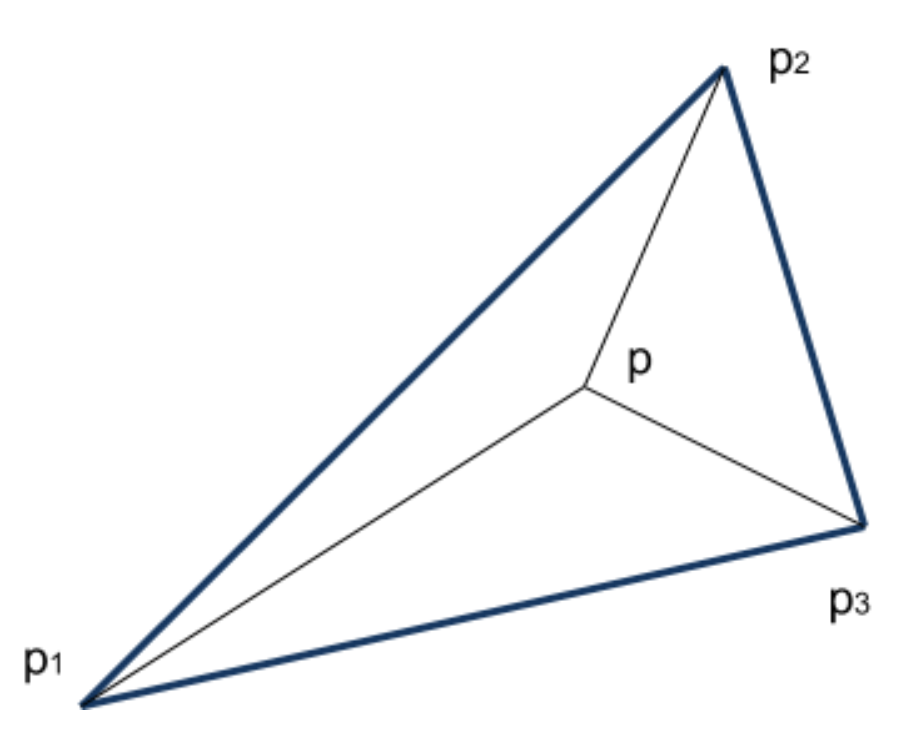
\includegraphics[width=0.9\textwidth]{triarea.png}
\end{minipage}

\begin{enumerate}[label=8g.\arabic*,start=3]

\item Udvid funktionen \texttt{colourAt} til at håndtere
  trekantsudvidelsen ved at implementere tricket nævnt ovenfor samt
  ved at benytte den implementerede funktion \lstinline{triarea2}.

\end{enumerate}

\begin{minipage}{.72\textwidth}

\begin{enumerate}[label=8g.\arabic*,start=4]

\item Lav en fil \texttt{figHouse.png}, der viser figuren
  \texttt{figHouse} i et $100\times150$ bitmap.

  Resultatet skulle gerne ligne figuren til højre.

\item Udvid funktionerne \texttt{checkFigure} og
  \texttt{boundingBox} fra øvelsesopgaverne til at håndtere
  udvidelsen.

  \texttt{boundingBox houseFig} skulle gerne give \texttt{((15, 10), (85,
    120))}.
\end{enumerate}

\end{minipage} \hfill \begin{minipage}{.2\textwidth}
  
\includegraphics[width=0.9\textwidth]{figHouse.png}
\end{minipage}

\noindent
Der skal laves black-box testing og in-code dokumentation af
funktionerne.

\vspace{1ex}

\noindent
Afleveringsopgaven skal afleveres som både \LaTeX, genererede
billedfiler, den genererede PDF, samt en fsx fil med løsningen for
hver delopgave, navngivet efter opgaven (f.eks.\ \texttt{8g-1.fsx}),
som kan oversættes med fsharpc, og hvis resultat kan køres med mono.
Det hele samles i en zip-fil med sædvanlig navnekonvention (se
tidligere ugesedler).

\LaTeX-rapporten skal vise de billedfiler, der bliver lavet i
opgaverne, og forklare ikke-oplagte designvalg i løsningerne af
opgaverne.

\vspace{1ex}

\hfill God fornøjelse

\end{document}

\newpage
\section*{Ugens nød 3}

Vi vil i denne uge stille en særligt udfordrende og sjov opgave,
som interesserede kan løse.  Det er helt frivilligt at lave denne
opgave, som vi kalder ``Ugens nød'', men der vil blive givet en
mindre præmie til den bedste løsning, der afleveres i Absalon.

\vspace{1ex}

Denne nød omhandler udvidelser/ændringer til datastrukturen for
geometriske funktioner, som er introduceret i øvelses og
afleveringsopgaverne herover.  Vi erstatter figurdatatypen med:

\begin{lstlisting}[numbers=none,frame=none,mathescape]
  type figure =
          | Circle of point * int * (colour * colour)
            // defined by center, radius, and centre/edge colours
          | Rectangle of point * point * (colour * colour * colour * colour)
            // defined by bottom-left corner, top-right corner,
            // and colours for each corner in the order (bl, br, tr, tl)
          | Mix of figure * figure
            // combine figures with mixed colour at overlap
          | Twice of figure * (int * int)
            // overlays figure with copy of self moved by vector
          | Ellipse of point * point * int * (colour * colour)
            // defined by two focal points and length of the great axis
            // with colours at each focal point
          | Triangle of point * point * point * (colour * colour * colour)
            // defined by three vertices and colours at these
\end{lstlisting}

\noindent
Vi har dels udvidet figurerne med ellipser og trekanter, og dels
ændret farverne fra at være ensartede henover en figur til at være
glidende overgange:

\begin{itemize}
\item I en cirkel skal farven variere lineært fra centrum til kant
  mellem de to specificerede farver.

\item I en rektangel eller trekant skal farverne variere, sådan at
  farverne i hjørnerne er som angivet, og farverne skifter glidende
  mellem disse henover det indre.  Angiv hvordan du definerer
  farveblandingen i et punkt.

  Et kvadrat med farverne sort, rød, gul og grøn i hjørnerne skulle
  gerne ligne billedet på side 1 i denne ugeseddel (men behøver ikke
  at være eksakt ligedan).

\item I en ellipse skal farverne i brændpunkterne være som angivet, og
  farven i resten af ellipsen skal afhænge af afstandende til de to
  brændpunkter.  Hvis de to afstande er lige store, skal farven
  blandes ligeligt, ellers skal farven afhænge af forholdet mellem de
  to afstande, sådan at farveovergangen er glidende.  Angiv formlen
  for farve baseret på forholdet mellem afstandende.

\item En trekant er korrekt, så længe farverne i hjørnerne er korrekt.

\item En ellipse er korrekt, hvis de to brændpunkter er forskellige,
  afstanden mellem brændpunkterne er skarpt mindre end storaksens
  længde, og de to farver er korrekte.

\end{itemize}

\noindent
Definer versioner af \texttt{colourAt}, \texttt{checkFigure}, og
\texttt{boundingBox}, der passer til den nye udgave af
\texttt{figure}, og følger de ovenstående retningslinjer.

Lav figurer, der afprøver glidende farveovergange samt korrekthed af
ovenstående funktioner.  Lav en rapport, der beskriver designvalg,
blandt andet til farveovergange og til at finde bounding-box for en
ellipse.  Bemærk, at en tæt bounding-box for en ellipse kan kræve
ikke-heltallige koordinater.  Disse skal rundes ned/op, sådan at
\texttt{boundingBox} returnerer den mindste kasse med heltallige
koordinater, der indeholder ellipsen.

Upload en zip-fil med \LaTeX-fil, PDF og .fsx filer.

Besvarelserne bliver bedømt på korrekthed, elegance, og på hvor godt
rapporten beskriver og begrunder designvalgene.

\end{document}
